% 文科固定来源第1页右栏Q26；保持不同于Q14的原图标号与投影。
% E/F为AA1/CC1中点，四棱锥底面顺序E-B-F-D1；不加入额外条件。
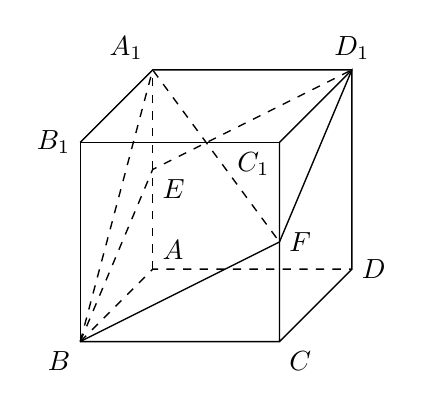
\begin{tikzpicture}[line width=0.5pt,scale=1.15]
  \coordinate (B) at (0,0);
  \coordinate (C) at (2.2,0);
  \coordinate (D) at (3,0.8);
  \coordinate (A) at (0.8,0.8);
  \coordinate (B1) at (0,2.2);
  \coordinate (C1) at (2.2,2.2);
  \coordinate (D1) at (3,3);
  \coordinate (A1) at (0.8,3);
  \coordinate (E) at (0.8,1.9);
  \coordinate (F) at (2.2,1.1);
  \draw (B)--(C)--(D)--(D1)--(C1)--(C);
  \draw (B)--(B1)--(C1);
  \draw (B1)--(A1)--(D1);
  \draw[dashed] (B)--(A)--(D);
  \draw[dashed] (A)--(A1);
  \draw (B)--(F)--(D1);
  \draw[dashed] (B)--(E)--(D1);
  \draw[dashed] (B)--(A1)--(F);
  \node[below left] at (B) {$B$};
  \node[below right] at (C) {$C$};
  \node[right] at (D) {$D$};
  \node[above right] at (A) {$A$};
  \node[left] at (B1) {$B_1$};
  \node[below left] at (C1) {$C_1$};
  \node[above] at (D1) {$D_1$};
  \node[above left] at (A1) {$A_1$};
  \node[below right] at (E) {$E$};
  \node[right] at (F) {$F$};
\end{tikzpicture}
